\section{Main window}
\label{sec:gui_main}
After starting the GUI, window (fig~\ref{fig:gui_main})
appears. It can be used to show other windows,
or to show status of devices and status of the running measurement.

\subsection{What to do here}
First setup TWM, AC source, DC meter, PJVS, than FR
measurement, run FR measurement, setup CE measurement, run CE measurement,
setup DG measurement, run DG measurement, SS measurement, run SS measurement.

\subsection{Elements of the window}
\begin{itemize}
	\item Button \texttt{About} --  shows a new window with informations on the software.
	\item Button \texttt{Setup TWM \& proc} -- shows a new window with settings for \texttt{TWM} and \texttt{GNU Octave}. % TODO link
	\item Button \texttt{Setup AC Source} -- shows a new window with settings for AC  % TODO link
	      source (sec.~\ref{sec:gui_acsrc}). The button \texttt{Manual control} right below shows a new % TODO link
	      independent window for direct manual control of an AC source (sec.~\ref{sec:gui_acsrc}).
	\item Button \texttt{Setup DC meter} -- shows a new window with settings for DC meter. % TODO link
	      The button \texttt{Manual control} right below shows a new % TODO link
	      independent window for direct manual control of a DC meter.
	\item Button \texttt{Setup PJVS} -- shows a new window with settings for PJVS. % TODO link
	      The button \texttt{Manual control} right below shows a new % TODO link
	      independent window for direct manual control of a PJVS.
	      % TODO add FR,CE,SS,DG
\end{itemize}

\begin{figure}
	\begin{center}
		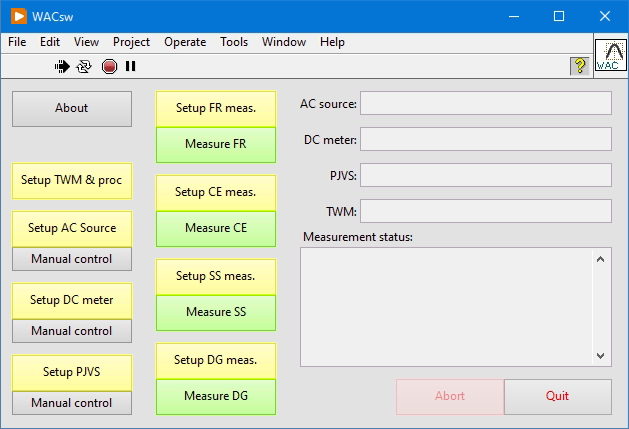
\includegraphics[width=0.95\textwidth]{fig_GUI/GUI_main.png}
	\end{center}
	\caption{Main GUI window.}
	\label{fig:gui_main}
\end{figure}

\section{AC Source}
\label{sec:gui_acsrc}

\subsection{Setup AC source}
The AC source is used for FR, CE and SS measurements. The setup is done using
window~\ref{fig:gui_acsrc_setup} (started from~\ref{sec:gui_main}).

\subsection{What to do here}
Setup AC source (type, VISA address), if the AC source needs to be referenced
by AC signal (e.g. FLuke calibrators), use checkbox \texttt{Synchronization by AC signal}
and setup source for the synchronization signal.
Check the settings by using button \texttt{Test connection}.

\subsection{Elements of the window}
\begin{itemize}
	\item Input \texttt{AC source type} --
	\item Input \texttt{VISA} --
	\item Input \texttt{Reference clock} --
	\item Checkbox \texttt{Synchronization by AC signal} --
	\item Button \texttt{Test connection} --
	\item Button \texttt{OK} --
	\item Button \texttt{Cancel} --
\end{itemize}

\begin{figure}
	\begin{center}
		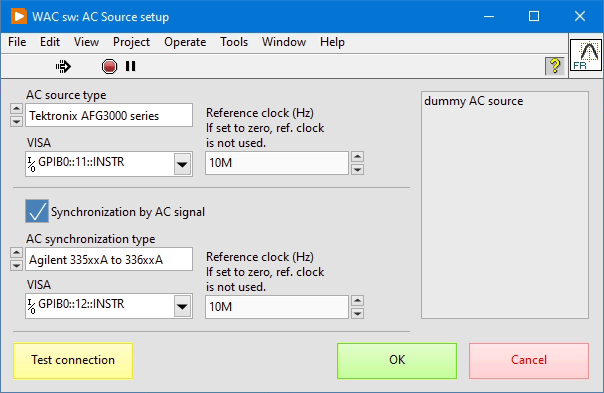
\includegraphics[width=0.95\textwidth]{fig_GUI/GUI_acsrc_setup.png}
	\end{center}
	\caption{Window to setup AC source.}
	\label{fig:gui_acsrc_setup}
\end{figure}

\subsection{Manual control of AC source}
The AC source can be controlled manually using window~\ref{fig:gui_acsrc_manual}.

What to do here: setup your AC source on the top left (if needed), if
\texttt{Synchronization by AC signal} is selected, setup also AC source on the
top right (checkbox \texttt{Synchronization by AC signal} in the right one has
no effect). Set required signal frequency, amplitude, ensure timeout is long
enough. Press \texttt{Initialize}, \texttt{Start}. Now AC source should be
generating signal. Press \texttt{Stop} to stop generation.

Elements of the window:
\begin{itemize}
	\item Element group for AC source --
	\item Element group for AC source used for Synchronization --
	\item Input \texttt{Signal frequency} --
	\item Input \texttt{Signal amplitude} --
	\item Input \texttt{General settings: Timeout value} --
	\item Box \texttt{Status} --
	\item Button \texttt{Initialize} --
	\item Button \texttt{Start} --
	\item Button \texttt{Stop} --
\end{itemize}

\begin{figure}
	\begin{center}
		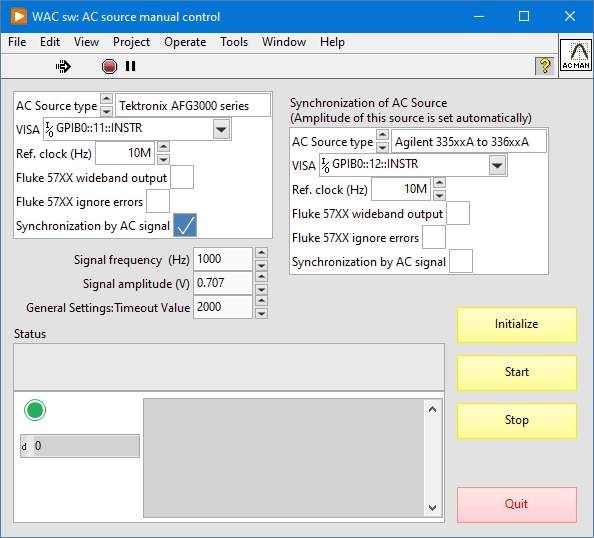
\includegraphics[width=0.95\textwidth]{fig_GUI/GUI_acsrc_manual.png}
	\end{center}
	\caption{}
	\label{fig:gui_acsrc_manual}
\end{figure}


\newpage
XXXXXXXXXXXXXXXXXXXXX
\newpage

\begin{figure}
	\begin{center}
		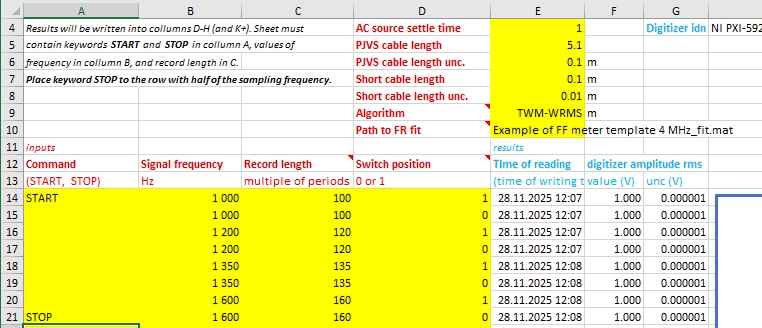
\includegraphics[width=0.95\textwidth]{fig_GUI/CE_template.png}
	\end{center}
	\caption{Piece-wise fit of a part of frequency response of a digitizer. The ligth red represents variations after using Monte Carlo method on the measured data and repeating fit. The vertical lines show boundaries of the pieces.}
	\label{fig:gui_ce_template}
\end{figure}

\begin{figure}
	\begin{center}
		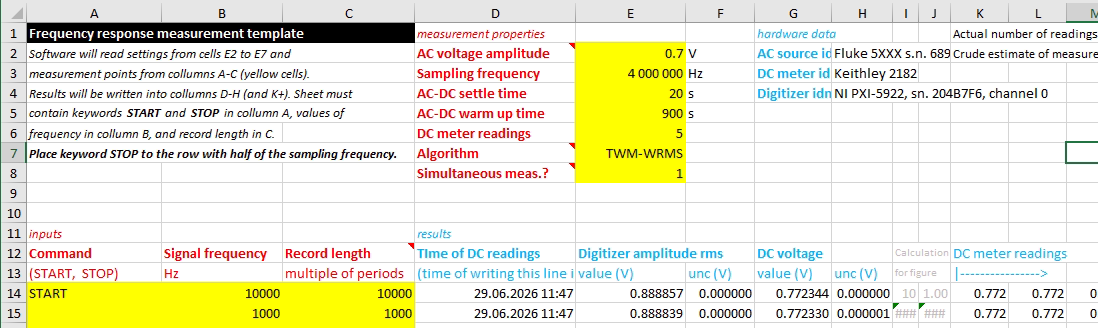
\includegraphics[width=0.95\textwidth]{fig_GUI/FR_template.png}
	\end{center}
	\caption{Piece-wise fit of a part of frequency response of a digitizer. The ligth red represents variations after using Monte Carlo method on the measured data and repeating fit. The vertical lines show boundaries of the pieces.}
	\label{fig:gui_fr_template}
\end{figure}

\begin{figure}
	\begin{center}
		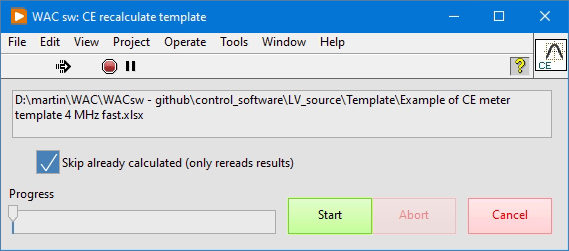
\includegraphics[width=0.95\textwidth]{fig_GUI/GUI_CE_recalculate.png}
	\end{center}
	\caption{Piece-wise fit of a part of frequency response of a digitizer. The ligth red represents variations after using Monte Carlo method on the measured data and repeating fit. The vertical lines show boundaries of the pieces.}
	\label{fig:gui_ce_recalculate}
\end{figure}

\begin{figure}
	\begin{center}
		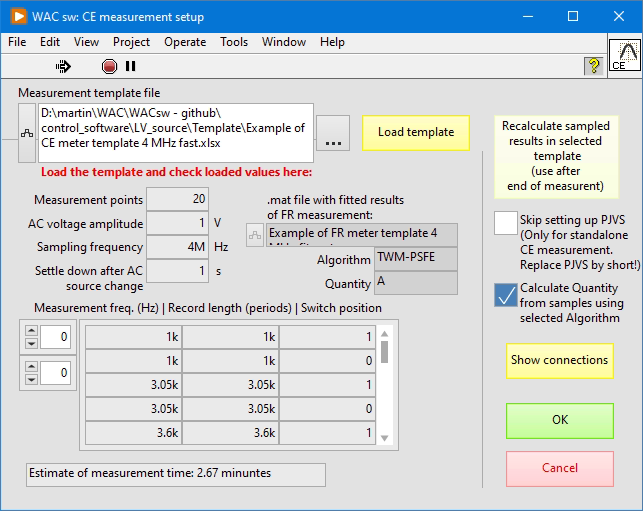
\includegraphics[width=0.95\textwidth]{fig_GUI/GUI_CE_setup.png}
	\end{center}
	\caption{Piece-wise fit of a part of frequency response of a digitizer. The ligth red represents variations after using Monte Carlo method on the measured data and repeating fit. The vertical lines show boundaries of the pieces.}
	\label{fig:gui_ce_setup}
\end{figure}

\begin{figure}
	\begin{center}
		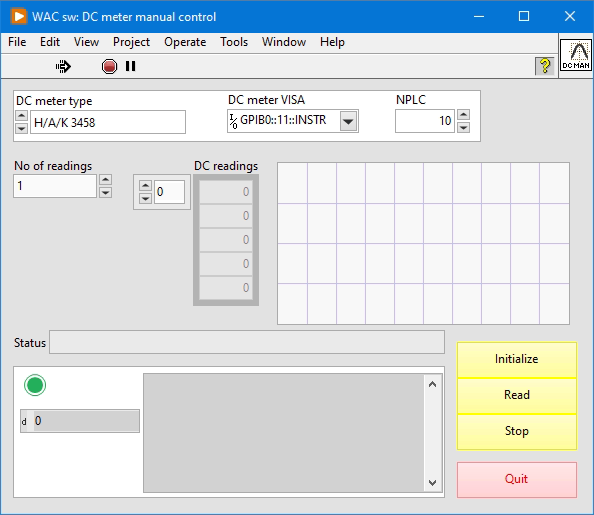
\includegraphics[width=0.95\textwidth]{fig_GUI/GUI_dcsrc_manual.png}
	\end{center}
	\caption{Piece-wise fit of a part of frequency response of a digitizer. The ligth red represents variations after using Monte Carlo method on the measured data and repeating fit. The vertical lines show boundaries of the pieces.}
	\label{fig:gui_dcsrc_manual}
\end{figure}

\begin{figure}
	\begin{center}
		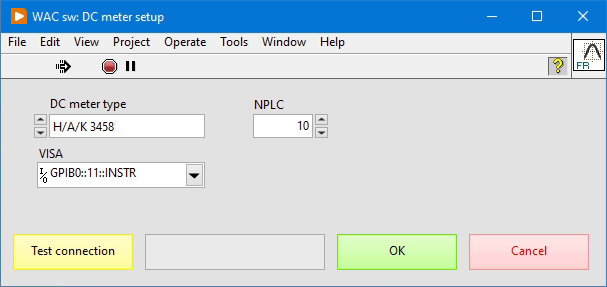
\includegraphics[width=0.95\textwidth]{fig_GUI/GUI_dcsrc_setup.png}
	\end{center}
	\caption{Piece-wise fit of a part of frequency response of a digitizer. The ligth red represents variations after using Monte Carlo method on the measured data and repeating fit. The vertical lines show boundaries of the pieces.}
	\label{fig:gui_dcsrc_setup}
\end{figure}

\begin{figure}
	\begin{center}
		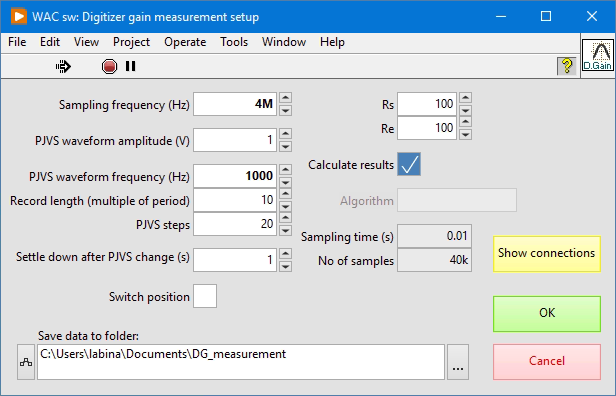
\includegraphics[width=0.95\textwidth]{fig_GUI/GUI_DG_setup.png}
	\end{center}
	\caption{Piece-wise fit of a part of frequency response of a digitizer. The ligth red represents variations after using Monte Carlo method on the measured data and repeating fit. The vertical lines show boundaries of the pieces.}
	\label{fig:gui_dg_setup}
\end{figure}

\begin{figure}
	\begin{center}
		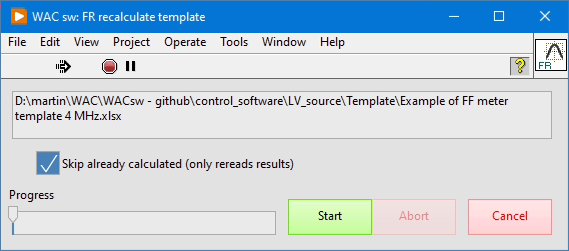
\includegraphics[width=0.95\textwidth]{fig_GUI/GUI_FR_recalculate.png}
	\end{center}
	\caption{Piece-wise fit of a part of frequency response of a digitizer. The ligth red represents variations after using Monte Carlo method on the measured data and repeating fit. The vertical lines show boundaries of the pieces.}
	\label{fig:gui_fr_recalculate}
\end{figure}

\begin{figure}
	\begin{center}
		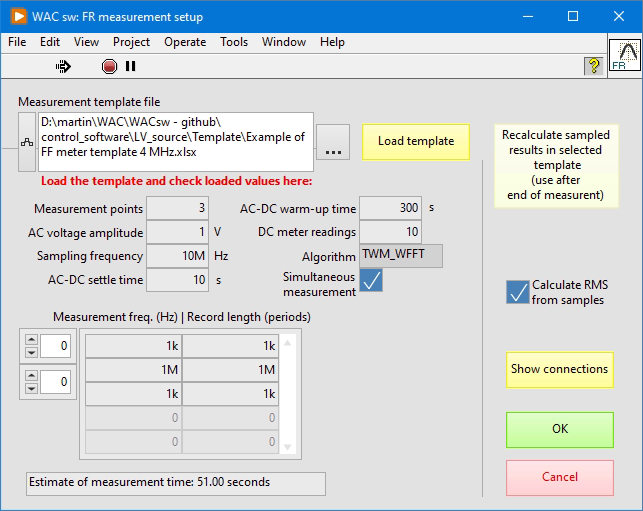
\includegraphics[width=0.95\textwidth]{fig_GUI/GUI_FR_setup.png}
	\end{center}
	\caption{Piece-wise fit of a part of frequency response of a digitizer. The ligth red represents variations after using Monte Carlo method on the measured data and repeating fit. The vertical lines show boundaries of the pieces.}
	\label{fig:gui_fr_setup}
\end{figure}

\begin{figure}
	\begin{center}
		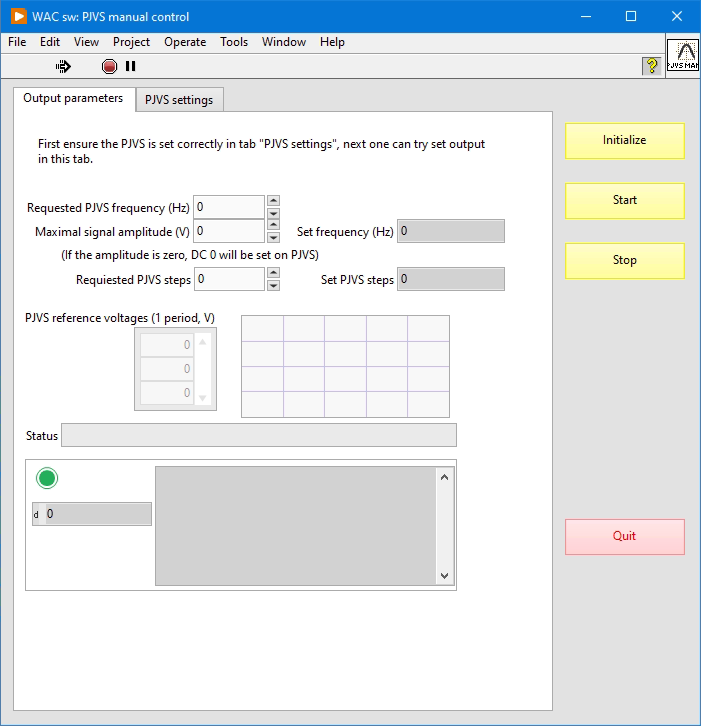
\includegraphics[width=0.95\textwidth]{fig_GUI/GUI_pjvs_manual.png}
	\end{center}
	\caption{Piece-wise fit of a part of frequency response of a digitizer. The ligth red represents variations after using Monte Carlo method on the measured data and repeating fit. The vertical lines show boundaries of the pieces.}
	\label{fig:gui_pjvs_manual}
\end{figure}

\begin{figure}
	\begin{center}
		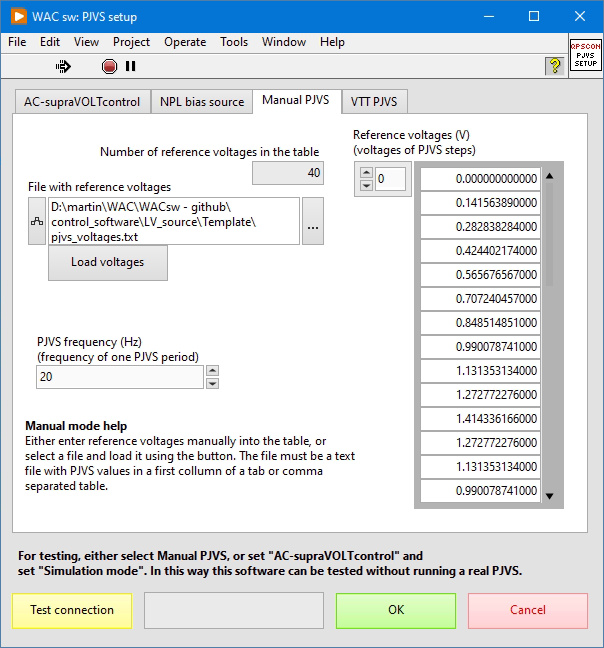
\includegraphics[width=0.95\textwidth]{fig_GUI/GUI_pjvs_setup_manual.png}
	\end{center}
	\caption{Piece-wise fit of a part of frequency response of a digitizer. The ligth red represents variations after using Monte Carlo method on the measured data and repeating fit. The vertical lines show boundaries of the pieces.}
	\label{fig:gui_pjvs_setup_manual}
\end{figure}

\begin{figure}
	\begin{center}
		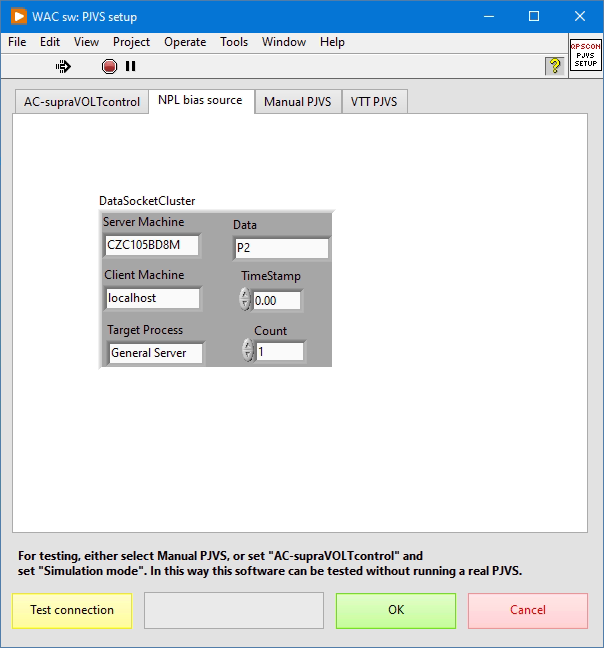
\includegraphics[width=0.95\textwidth]{fig_GUI/GUI_pjvs_setup_npl.png}
	\end{center}
	\caption{Piece-wise fit of a part of frequency response of a digitizer. The ligth red represents variations after using Monte Carlo method on the measured data and repeating fit. The vertical lines show boundaries of the pieces.}
	\label{fig:gui_pjvs_setup_npl}
\end{figure}

\begin{figure}
	\begin{center}
		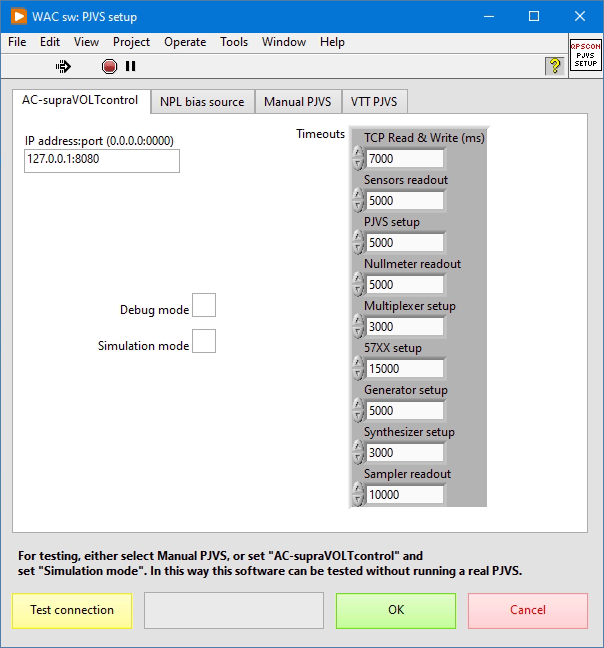
\includegraphics[width=0.95\textwidth]{fig_GUI/GUI_pjvs_setup_supracon.png}
	\end{center}
	\caption{Piece-wise fit of a part of frequency response of a digitizer. The ligth red represents variations after using Monte Carlo method on the measured data and repeating fit. The vertical lines show boundaries of the pieces.}
	\label{fig:gui_pjvs_setup_supracon}
\end{figure}

\begin{figure}
	\begin{center}
		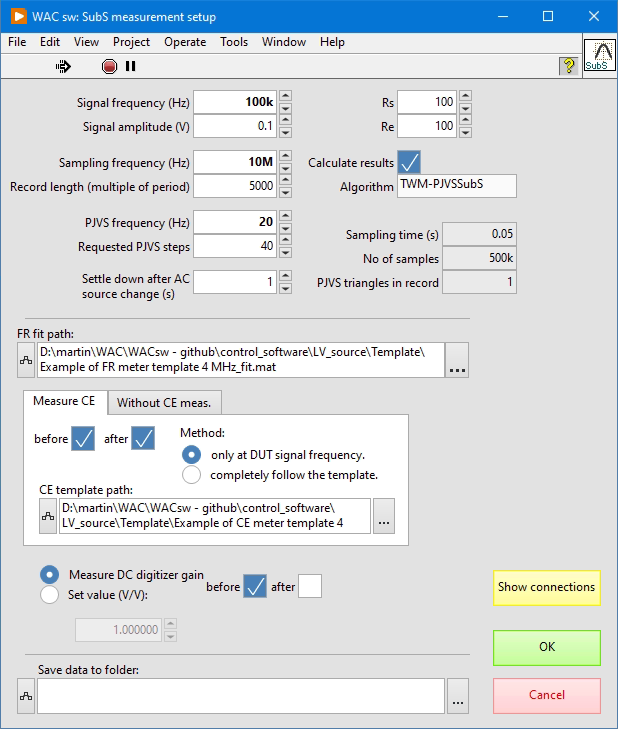
\includegraphics[width=0.95\textwidth]{fig_GUI/GUI_SS_setup_withCEmeas.png}
	\end{center}
	\caption{Piece-wise fit of a part of frequency response of a digitizer. The ligth red represents variations after using Monte Carlo method on the measured data and repeating fit. The vertical lines show boundaries of the pieces.}
	\label{fig:GUI_SS_setup_withCEmeas}
\end{figure}

\begin{figure}
	\begin{center}
		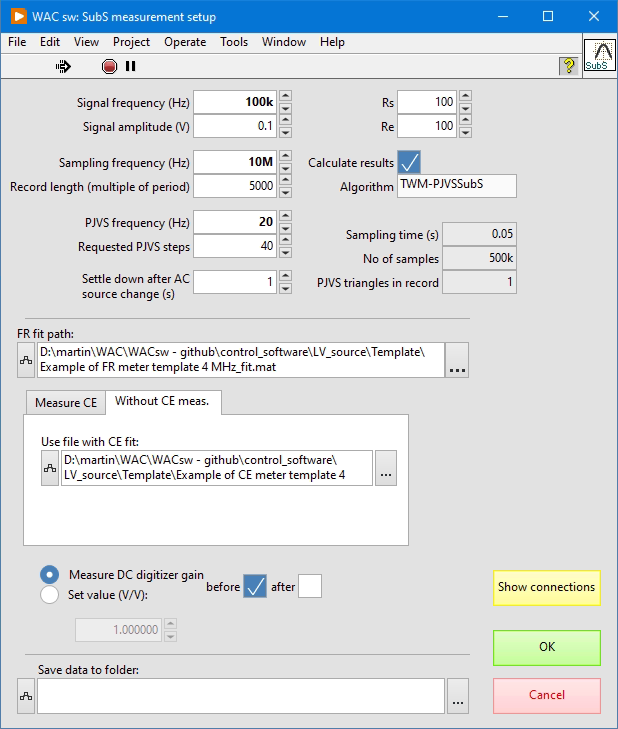
\includegraphics[width=0.95\textwidth]{fig_GUI/GUI_SS_setup_withoutCEmeas.png}
	\end{center}
	\caption{Piece-wise fit of a part of frequency response of a digitizer. The ligth red represents variations after using Monte Carlo method on the measured data and repeating fit. The vertical lines show boundaries of the pieces.}
	\label{fig:GUI_SS_setup_withoutCEmeas}
\end{figure}

\begin{figure}
	\begin{center}
		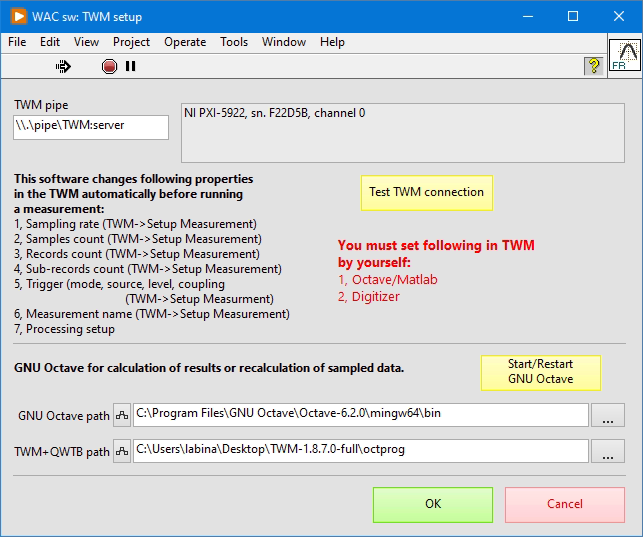
\includegraphics[width=0.95\textwidth]{fig_GUI/GUI_twm_setup.png}
	\end{center}
	\caption{Piece-wise fit of a part of frequency response of a digitizer. The ligth red represents variations after using Monte Carlo method on the measured data and repeating fit. The vertical lines show boundaries of the pieces.}
	\label{fig:gui_twm_setup}
\end{figure}
